\section{Data}

\begin{figure}
    \centering
    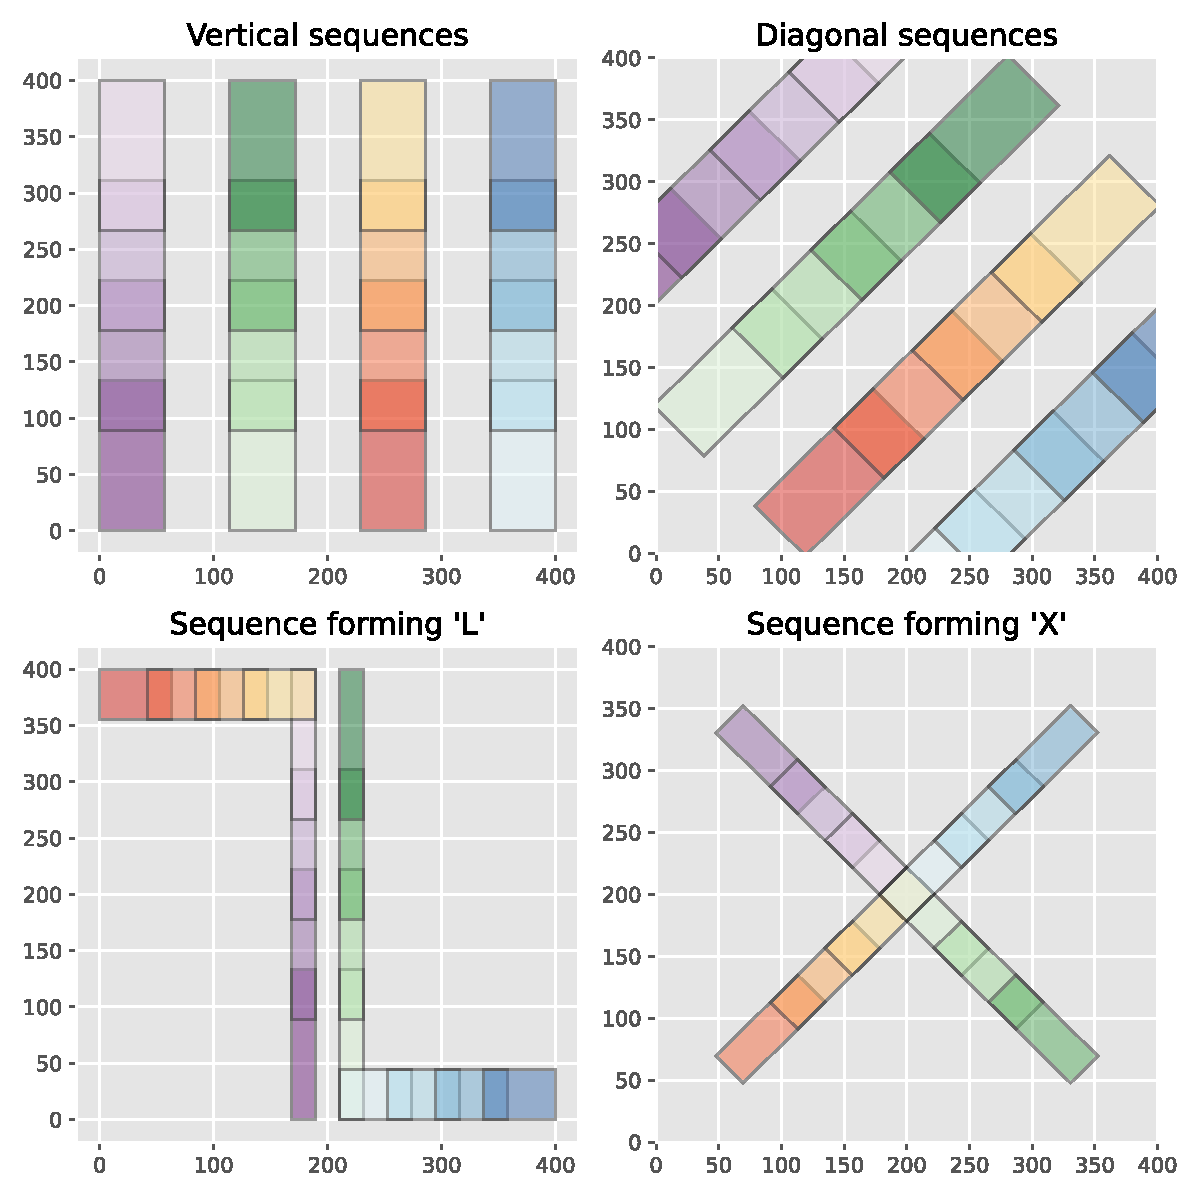
\includegraphics[width = \textwidth]{src/imgs/generated-datasets.pdf}
    \caption{Source: elaborated by author. Generated datasets, each rectangle represents an event, the colors are only indicative of "groups" of events. }
    \label{fig:generated-datasets}
\end{figure}
To evaluate the method and also demonstrate its applicability, it was made a selection of generated datasets and available spatio-temporal datasets.
%

\subsection{Generated datasets}

The intention of the generated datasets is to create simple patterns and verify the representation of this pattern in the generated visualization,
%
and also present examples that highlight the good properties of the presented method.
%
With that in mind, datasets shown in Fig.~\ref{fig:generated-datasets} were created by the repetition of simple shapes, rectangles whose center calculations are easy, areas, and intersection areas. The events created do not have a time attribute.
%

As shown in Figure~\ref{fig:generated-datasets}, it is possible to identify that are "columns" of events intersecting each other, these columns are also marked by color. 
%
These columns evaluate if the projections and the intersection adjustment will keep events from the same column together and if objects from different columns will intersect each other.
%
These datasets will be available to select on the evaluation tool previously presented.

\subsection{Real world dataset}

The real-world data is from the Waze app.
%
The data collected from the app are alerts created from users to notify accidents, roadwork, traffic changes from the city of Rio de Janeiro.
%
The available data is from a longer period of time, and different subsets can be created by selecting the time interval.
%
Each row of data contains information about: identification of the alert, date with hour and minutes, position (longitude, latitude), type, subtype, a comment explaining the alert, number of likes, reliability, and confidence of the alert.
%
There are many alerts each day, but much of the data is a repetition of the same alert with different timestamps. 
%
It was used two subsets of the data, in both cases only considering alerts where the user add a commentary explaining it, the first subset is from the interval of 1/12/18 to 31/03/19, the second is only from the month of February of 2019.
%
The first one is going to be present in the use-case~\ref{sec:use-case}, and the second is used on the examples figures in the Section~\ref{sec:visualization-tool}.
%
A general overview of the datasets is available at Figs.~\ref{fig:waze-overview}.

\begin{figure}
    \centering
    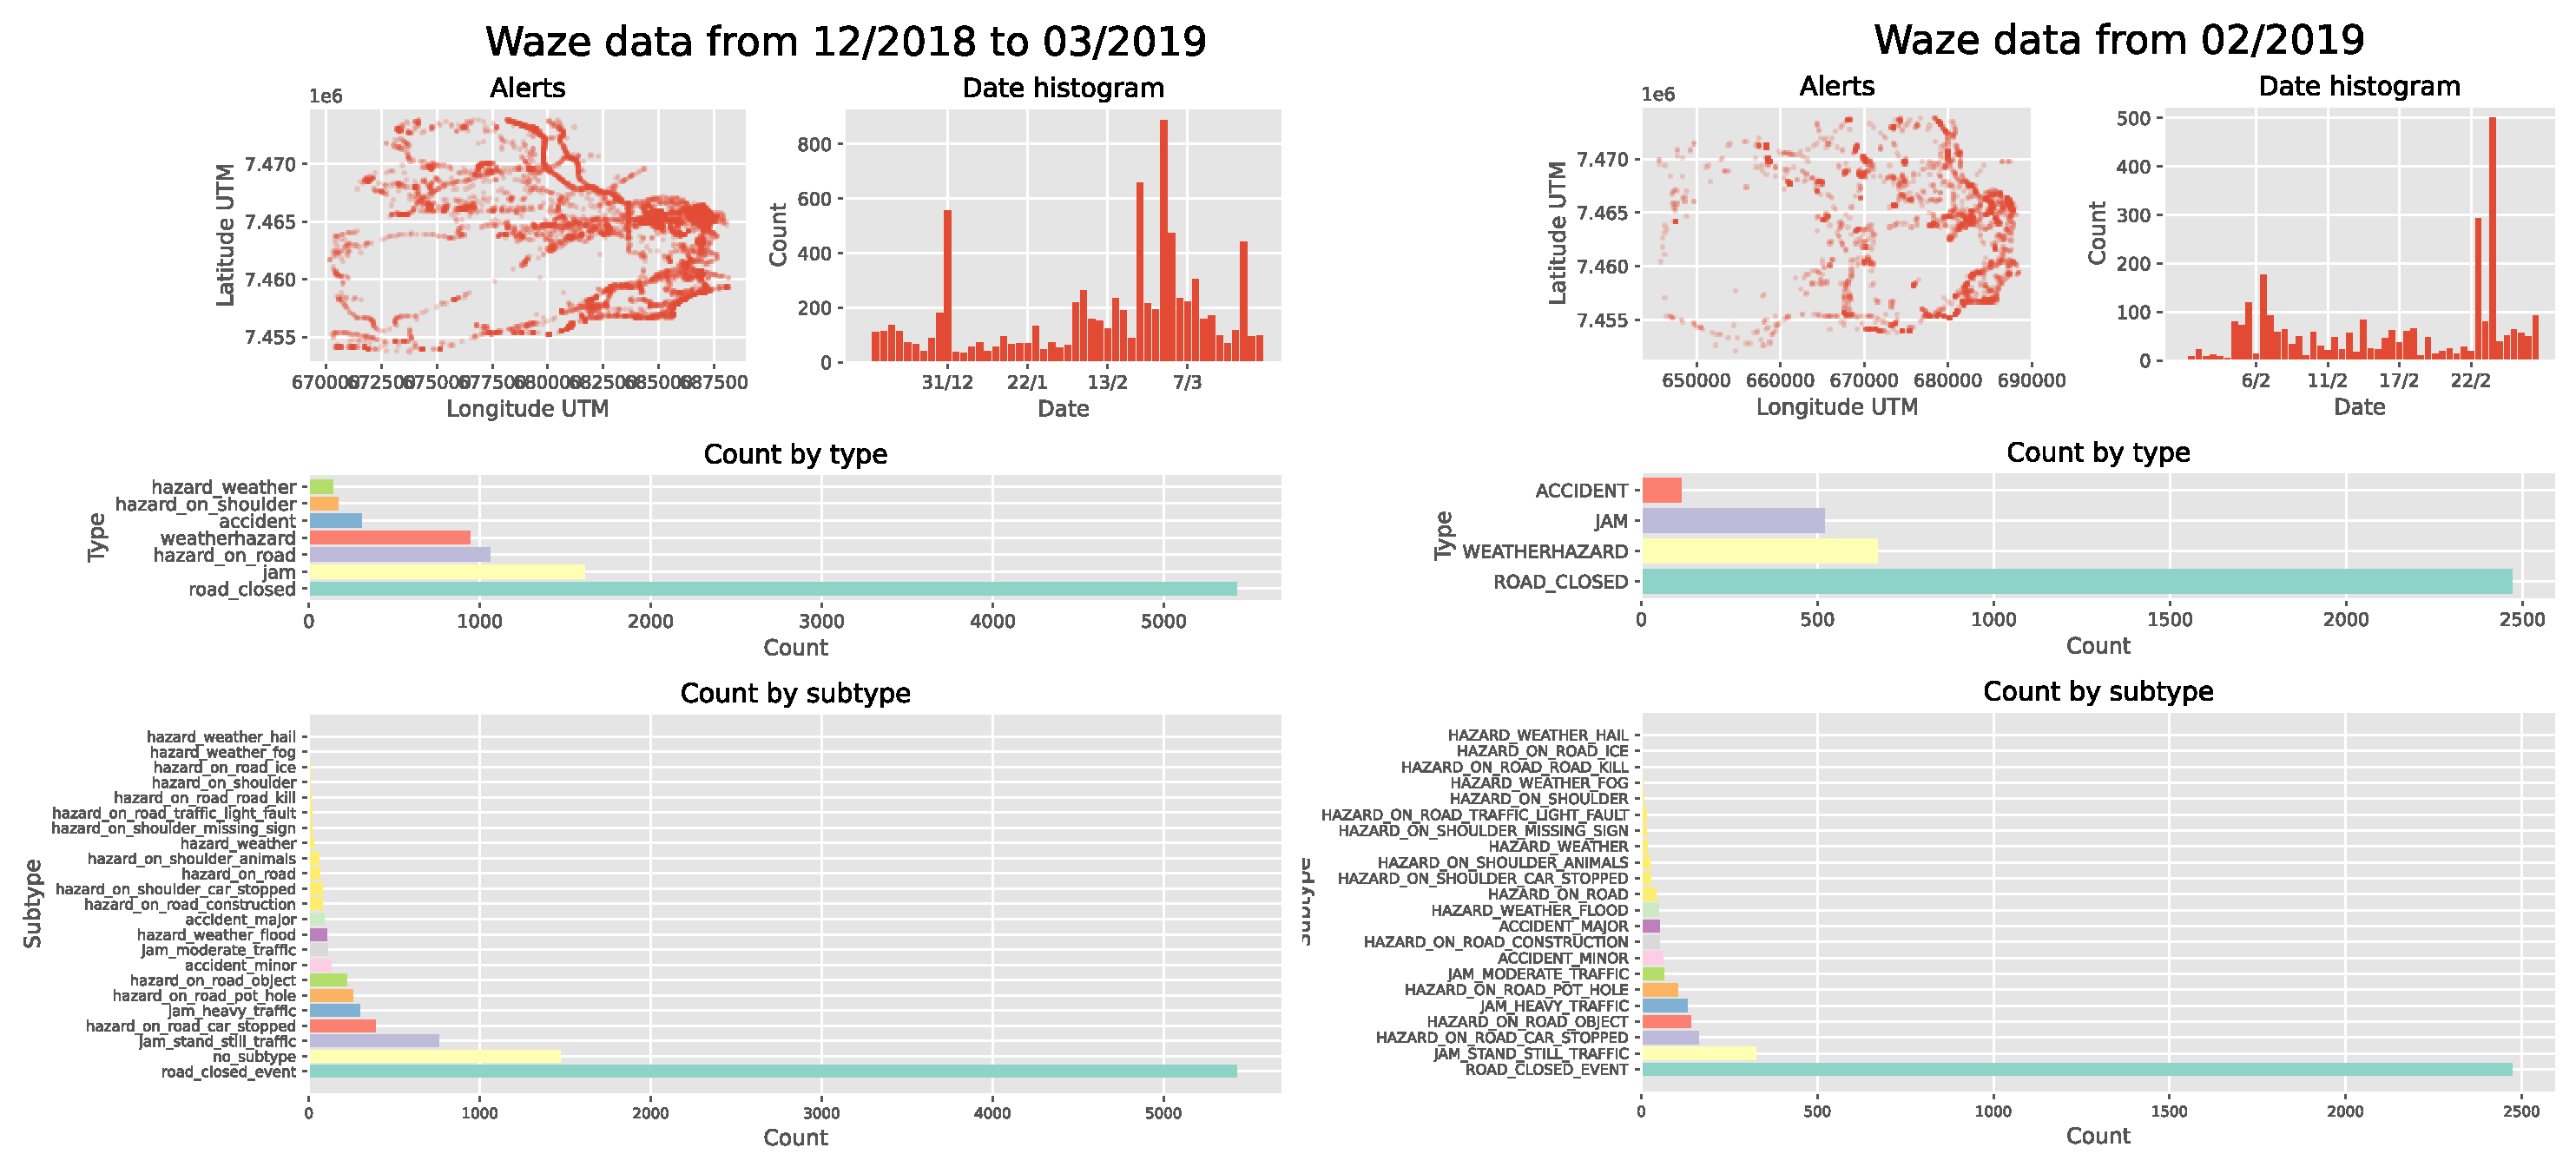
\includegraphics[width = \textwidth]{src/imgs/waze-datasets.pdf}
    \caption{Source: elaborated by author. General characteristics from Waze dataset on both subsets, with spatial distribution, temporal histogram, and distribution by type and subtype of alerts.}
    \label{fig:waze-overview}
\end{figure}


To transform this dataset into events it is necessary to apply a clustering algorithm,
%
each cluster of points from a specific spatial region in a time interval can be generated by an urban event in the city, 
%
such as an accident, the carnival festivities, roadwork.
%
The clustering algorithm will be the ST-DBSCAN presented in section \ref{sec:clustering} with small changes.

%
The initial change is that the parameter $\Delta \varepsilon$ is not used. 
%  
Another adaptation is to consider points with temporal duration. Let $p \in D$, it is defined the points $p_{t0}$ and $p_{t1}$ with same spatial position and different temporal values, $p$ is the segment that connects $p_{t0}$ and $p_{t1}$. The temporal neighborhood of $p$ is the interval $[p_{t0} - Eps_2, p_{t1} + Eps_2]$. The neighborhood is exemplified in Figure \ref{fig:stdbscan_neighborhood}.

\begin{figure}
    \centering
    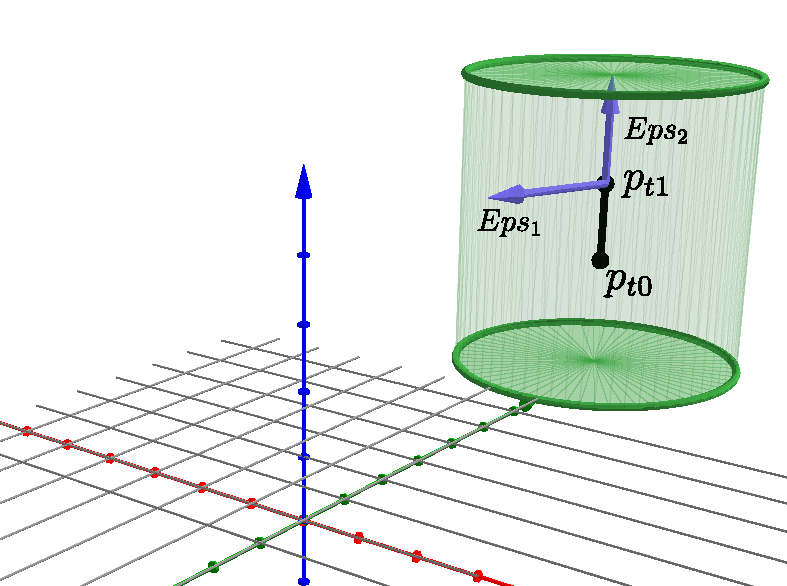
\includegraphics[width = 8cm]{src/imgs/point_neighborhood_stdbscan.pdf}
    \caption{Source: Elaborated by author. Example of point neighborhood, the point is actually a segment perpendicular to the plane $XY$, from points $p_{t0}$ to $p_{t1}$, the green cylinder is the neighborhood, the form is because of the quadratic distance in the spatial dimension and the linear distance in time.} 
    \label{fig:stdbscan_neighborhood}
\end{figure}

 
%
The last adaptation is the use of another attribute called \textit{subtype}, points will be in the same neighborhood if their values for \textit{subtypes} are equal. 

%
To compute spatial neighborhoods it will be used the euclidean distance, for that it is necessary to project the coordinates to the UTM system,
%
because in small regions it is a good approximation of a planet's surface and the distances can be computed with the euclidean formula.
%
The neighborhood size parameters used in the examples are selected by testing, with a set of parameters values, in each one it was computed the clustering and the result was analyzed with the visualization tool~\ref{sec:visualization-tool}, verifying if the points from the same cluster are coherent.

%
%The algorithm for retrieving neighbors considering the implement changes is at \ref{alg:retrieve_neighbors}.

%\begin{algorithm}[H]
%\label{alg:retrieve_neighbors}
%\SetAlgoLined
%\SetKwInOut{Input}{Input}
%\Input{
%$p$ - point with attributes \\
%$Eps_1$ - threshold for spatial distance in neighborhood \\
%$Eps_2$ - threshold for temporal distance in neighborhood \\
%}
%\SetKwInOut{Output}{Output}
%\Output{
%$N$ - subset of points in the neighborhood
%}
%\tcc{find all points from $D$ that are inside the circle of center $p$ and radium $Eps_1$} 
%$N = $ kdtree\_query$(p, Eps_1)$\;
%\tcc{find all points from $N$ that are inside the segment of %temporal neighborhood}
%$N = $ temporal\_query$(p, N, Eps_2)$\;
%\tcc{find all points from $N$ of same subtypes}
%$N = $ subtype\_query$(p, N)$\;
%\caption{Algorithm for retrieving neighbors of point $p$ in the %ST-DBSCAN algorithm.}
%\end{algorithm}

